\chapter{Operador de agregación Krum}\label{sec:krum}
Un problema común que nos encontraremos más adelante es el de agregar una serie de estimaciones de un gradiente para obtener un nuevo vector que nos permita resumir la información contenida por los vectores anteriores. Esto es, obtener una estimación del gradiente de una función mediante estimaciones previas en un algoritmo iterativo.

En nuestro caso podemos considerar que tenemos $n$ vectores, de los cuales $f$ pueden ser bizantinos, esto es, con valores arbitrarios. En cada paso $t$ de nuestro algoritmo, se considera un vector real denotado por $x_t \in \mathbb{R}^d$ de parámetros. Cada vector consiste en un valor estimado $V_p^t=G(x_t, \xi_p^t)$ del gradiente $\nabla Q(x_t)$ de la función de coste $Q$, donde $\xi_p^t$ es una variable aleatoria representando una muestra de un conjunto de datos. Sin embargo, un vector bizantino $V_b^t$ se puede desviar arbitrariamente del vector esperado.

Dadas las estimaciones podemos calcular un nuevo vector $F(V_1^t, \ldots, V_n^t)$ mediante una función determinista $F: (\mathbb{R}^d)^n \to \mathbb{R}^d$ llamada regla de agregación y los vectores estimados. Finalmente, podemos actualizar nuestros parámetros mediante la siguiente ecuación basada en el descenso estocástico por el gradiente
\begin{equation}
	x_{t+1} = x_{t} - \eta_t \cdot F(V_1^t, \ldots, V_n^t).
\end{equation}

\begin{figure}[h]
    \centering
    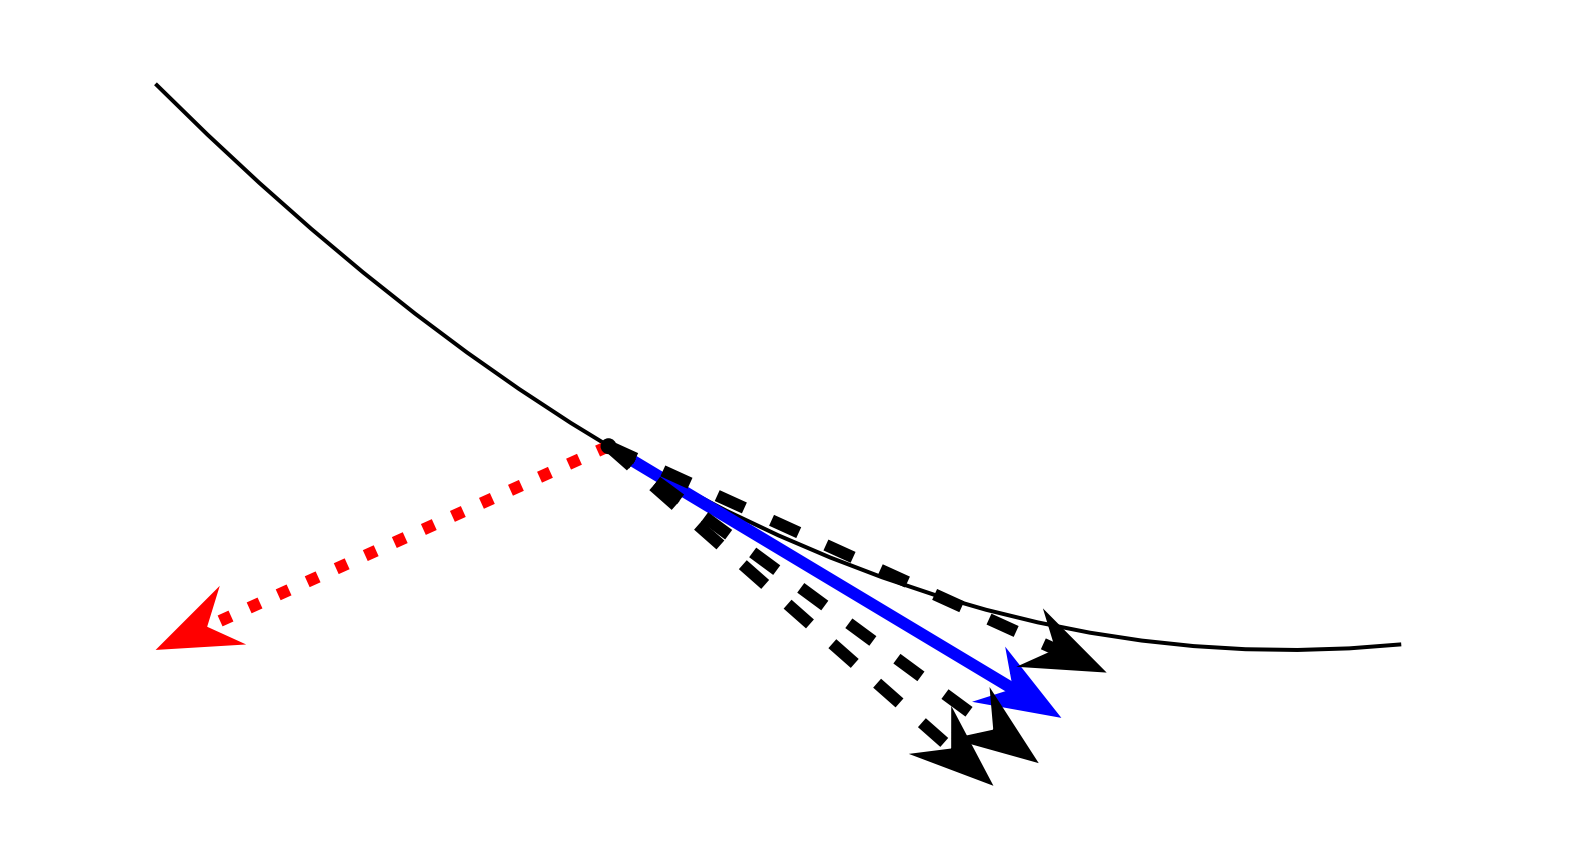
\includegraphics[width=0.8\textwidth]{figuras/krum_gradient.png}
    \caption{Las estimaciones del gradiente producidas por los estimadores correctos (flechas discontinuas negras) están distribuidas alrededor del gradiente (flecha azul sólida). Un vector bizantino puede tener un valor arbitrario (flecha roja discontinua). Fuente: \cite{krum-2017}.}
    \label{fig:krumgradient}
\end{figure}

Esperamos que los vectores no bizantinos (benignos) sean estimaciones insesgadas del gradiente $\nabla Q(x_t)$.  De manera más precisa, en cada ronda $t$, los vectores benignos $V_i^t$ son vectores aleatorios \ac{i.i.d.} con $V_i^t \sim G(x_t, \xi_i^t)$ tales que $E_{\xi_i^t}[G(x_t, \xi_i^t)] = \nabla Q(x_t)$. 

Como veremos más adelante en esta memoria, la regla de agregación más común consiste en calcular la media de los vectores. Sin embargo, ninguna combinación lineal de los vectores puede tolerar a un vector bizantino, y por tanto esta regla no es resistente a ataques bizantinos.

\begin{lemma}
	Sea $F_{lin}$ una regla de agregación de la forma $F_{lin}(V_1, \ldots, V_n)=\sum_{i=1}^n \lambda_i \cdot V_i$ donde $\lambda_i$ son escalares distintos de cero. Sea $U \in \mathbb{R}^d$. Entonces, un solo vector bizantino puede hacer que $F$ siempre compute $U$ como salida. Particularmente, un único vector bizantino puede evitar la convergencia del modelo. 
\end{lemma}

\begin{proof}
	La demostración resulta inmediata. Dado que se puede asumir que se tiene conocimiento total sobre los vectores $V_i$ y la regla de agregación $F_{lin}$ (y por tanto de los escalares $\lambda_i$), puede proponer el el vector $V_n = \frac{1}{\lambda_n}\cdot U - \sum_{i=1}^{n-1}\frac{\lambda_i}{\lambda_n}V_i$, haciendo así que $F_{lin}(V_1, \ldots, V_n)=U$.
\end{proof}

Viendo esto, nuestro objetivo es buscar una regla de agregación resistente a ataques bizantinos. De manera intuitiva, queremos que el resultado (esperado) $F$  de nuestra regla no se aleje demasiado del gradiente ''real'' $g$. Esto se puede expresar mediante el uso de una cota inferior del producto escalar del vector $F$ y $g$, así acotando el ángulo que ambos forman. Particularmente, si $E[F]$ se encuentra en una bola centrada en $g$ con radio $r$, entonces el producto escalar está acotado inferiormente por un término que implica a $\sin \alpha = r / ||g||$.

Otra condición que buscamos, aunque más técnica, es que los momentos de $F$ deben de depender de los momentos del estimador (correcto) del gradiente $G$. Esto se debe a que las cotas de los momentos de $G$ se suelen usar para controlar los efectos de la naturaleza discreta del método del descenso estocástico por el gradiente.

\begin{definition}
	Sea $0 \le \alpha < \pi/2$ cualquier ángulo, y cualquier entero $0 \le f \le n$. Sean $V_1, \ldots, V_n$ vectores aleatorios \ac{i.i.d.} en $\mathbb{R}^d$, $V_i \sim G$, con $E[G]=g$. Sean $B_1, \ldots, B_f$ vectores aleatorios en $\mathbb{R}^d$, posiblemente dependientes de los vectores $V_i$. Diremos que una regla de agregación $F$ es $(\alpha, f)$-Resistente bizantina si, para cualesquiera $1 \le j_1 < \ldots < j_f \le n$, el vector
	\begin{equation}
		F = F(V_1, \dots, \underbrace{B_1}_{j_1}, \ldots, \underbrace{B_f}_{j_f}, \ldots, V_n)
	\end{equation}
	cumple que $\langle E[F], g \rangle \ge (1-\sin \alpha) \cdot ||g||^2 > 0$ y que para $r \in \{ 2, 3, 4\}$, $E[||F||^r]$ está superiormente acotada por una combinación linear de los términos $E[||G||^1], \ldots, E[||G||^{r_{n-1}}]$ con $r_1 + \ldots + r_{n-1}=r$.
\end{definition}

\begin{figure}[h]
    \centering
    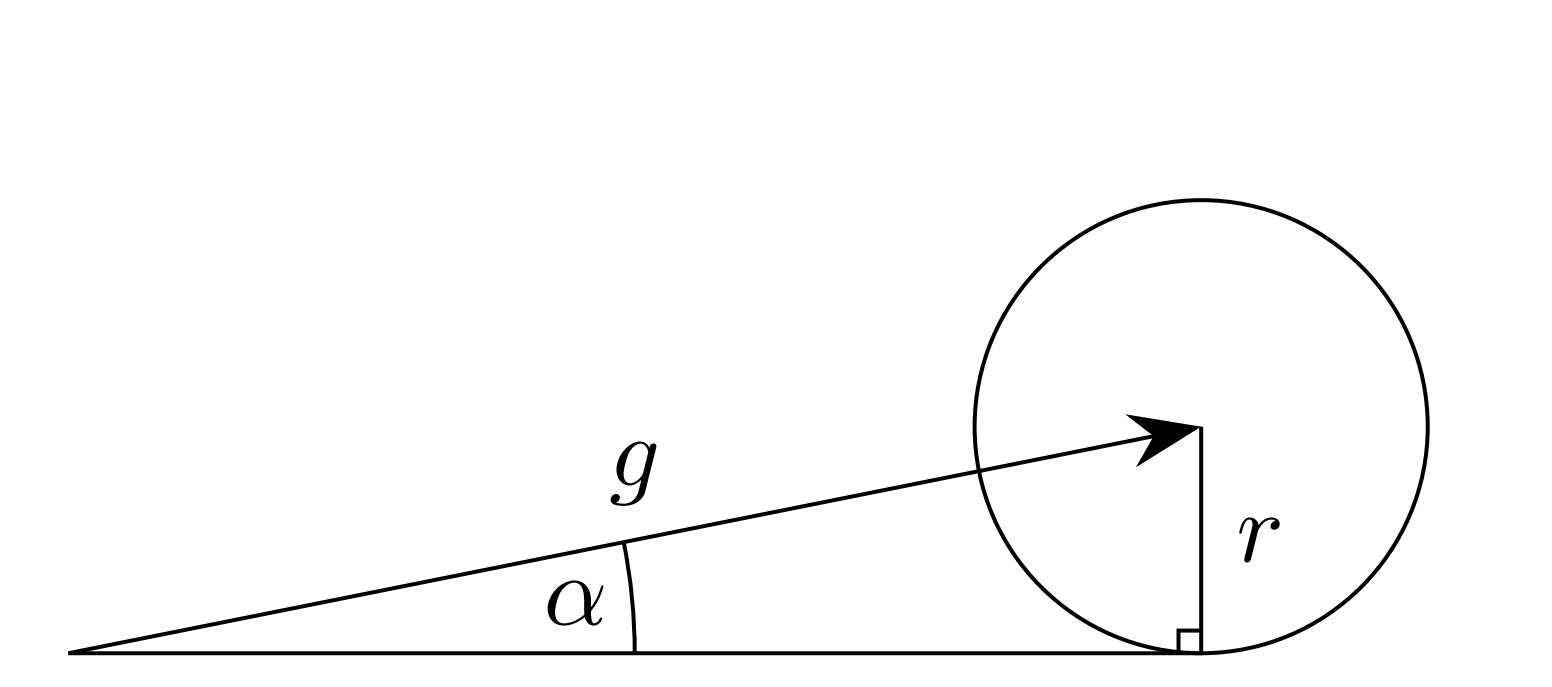
\includegraphics[width=0.8\textwidth]{figuras/krum_angle.png}
    \caption{Si $||E[F-g]|| \le r$, entonces $\langle E[F], g \rangle$ está inferiormente acotado por $(1- \sin \alpha)||g||^2$ donde $\sin \alpha= r/ ||g||$. Fuente: \cite{krum-2017}.}
    \label{fig:krumangle}
\end{figure}

Tras haber dado una definición formal de lo que es una regla de agregación resistente, procedemos a introducir la regla de agregación Krum, que cumplirá la condición ya explicada. La idea detrás de Krum consiste en que calcular el promedio puede verse también como calcular el vector que minimiza la suma de las distancias al cuadrado de los vectores $V_i$. La idea de Krum vuelve a ser la de encontrar un vector que minimice sumas de distancias a los demás vectores, pero excluyendo de estas a los vectores que estén ´´muy lejos´´ de manera que un vector bizantino no pueda forzar a la regla a escoger un vector arbitrario.

Formalmente, se define la regla de agregación Krum $KR(V_1, \ldots, V_n)$ de la siguiente manera. Para todos $i \ne j$, denotamos por $i \to j$ el hecho de que el vector $V_j$ está en el conjunto de los $n-f-2$ vectores más cercanos a $V_i$. Para cada vector $i$ se define la siguiente puntuación
\begin{equation}
	s(i) = \sum_{i \to j} ||V_i - V_j||^2.
\end{equation}
Finalmente, $KR(V_1, \ldots, V_n) = V_{i_*}$ donde $s(i_*) \le s(i)$ para todo $i$.

A continuación daremos una condición sobre $n$, $f$ y el estimador del gradiente usado para que la regla Krum sea $(\alpha, f)$-resistente bizantina.

\begin{theorem}
	Sean $V_1, \ldots, V_n$ vectores aleatorios $d$-dimensionales \ac{i.i.d.} tales que $V_i \sim G$ con $E[G]=g$ y $E[||G-g||^2]=d\sigma^2$. Sean $B_1, \ldots, B_f$ vectores aleatorios, posiblemente dependientes de los vectores $V_i$. Si $2f + 2 < n$ y $\eta(n, f)\sqrt{d}\cdot \sigma < ||g||$, donde
	\begin{equation}
		\eta(n,f) = \sqrt{2 \left( n-f + \frac{f \cdot (n-f-2) + f^2 \cdot(n-f-1)}{n-2f-2} \right)},
	\end{equation}
	
	entonces la regla de agregación Krum $KR$ es $(\alpha, f)$-resistente bizantina, donde el $\alpha$ se define como
	\begin{equation}
		\sin \alpha = \frac{\eta(n, f) \cdot \sqrt{d} \sigma}{||g||}.
	\end{equation}
\end{theorem}

\begin{proof}
	Sin perder generalidad, podemos asumir que los vectores $B_1, \ldots, B_f$ ocupan las últimas $f$ posiciones de la lista de argumentos de $KR$. Diremos que un índice es correcto si se refiere a un vector entre $V_1, \ldots, V_{n-f}$ y bizantino si se refiere a un vector entre $B_1, \ldots, B_f$. Para cada índice $i$, denotamos por $\delta_c(i)$  (o $\delta_b(i)$) a la cantidad de índices correctos (o bizantinos) $j$ tales que $i \to j$. Claramente tenemos que
	\begin{equation}\begin{split}
			\delta_c(i) + \delta_b(i) = n - f - 2 \\
			n - 2f - 2 \le \sigma_c(i) \le n-f-2 \\
			\sigma_b(i) \le f.
	\end{split}\end{equation}
	
	Nos centraremos primero en acotar el producto escalar. Empezaremos dando una cota superior de $||E[KR - g]||^2$. Recordemos que, si $j$ es correcto, entonces $E[V_j]=g$. Sea $i_*$ el índice del vector elegido por la regla Krum.
	\begin{equation}\begin{split}
			||E[KR-g]||^2 \le ||E \left( KR - \frac{1}{\delta_c(i_*)} \sum_{i_* \to j \text{ correctos}}V_j \right) ||^2 \\
			\le E[|| KR - \frac{1}{\delta_c(i_*)} \sum_{i_* \to j \text{ correctos}}V_j ||^2] \quad \text{(Desigualdad de Jensen)} \\
			\le \sum_{i \text{ correcto}} E[|| KR - \frac{1}{\delta_c(i_*)} \sum_{i_* \to j \text{ correctos}}V_j ||^2]  \mathbb{1}(i_* = i) \\
			+ \sum_{k \text{ biz}} E[||B_k - \frac{1}{\delta_c(k)} \sum_{k \to j \text{ correctos}}V_j||^2] \mathbb{1}(i_*=k)
	\end{split}\end{equation}
	
	Ahora analizamos el caso $i_* = i$ con $i$ un índice correcto.
	\begin{equation}\begin{split}
			||V_i - \frac{1}{\delta_c(i)}\sum_{i_* \to j \text{ correctos}}V_j||^2 = ||\frac{1}{\delta_c(i)}\sum_{i_* \to j \text{ correctos}}V_i - V_j||^2 \\
			\le \frac{1}{\delta_c(i)}\sum_{i_* \to j \text{ correctos}}||V_i - V_j||^2
	\end{split}\end{equation}
	
	y por tanto
	\begin{equation}\begin{split}
			E[||V_i - \frac{1}{\delta_c(i)}\sum_{i_* \to j \text{ correctos}}V_j||^2] \le \frac{1}{\delta_c(i)}\sum_{i_* \to j \text{ correctos}}E[||V_i - V_j||^2] \\
			\le 2d \sigma^2.
	\end{split}\end{equation}
	Ahora analizamos el caso $i_*=k$ siendo $k$ un índice bizantino. El hecho de que $k$ minimiza la puntuación significa que para todos los índices correctos $i$
	\begin{equation}\begin{split}
			\sum_{k \to j \text{ correctos}} ||B_k - V_j||^2 + \sum_{k \to l \text{ bizantinos}} ||B_k - B_l||^2 \\
			\le \sum_{i \to j \text{ correctos}} ||V_i - V_j||^2 + \sum_{i \to l \text{ bizantinos}} ||V_i - B_l||^2.
	\end{split}\end{equation}
	Entonces, para todo índice correcto $i$
	\begin{equation}\begin{split}
			||B_k - \frac{1}{\delta_c(k)} \sum_{k \to j \text{ correctos}}V_j||^2 \le \frac{1}{\delta_c(k)}\sum_{k \to j \text{ correctos}} ||B_k - V_j||^2 \\
			\le \frac{1}{\delta_c(k)}\sum_{i \to j \text{ correctos}} ||V_i - V_j||^2 + \frac{1}{\delta_c(k)} \underbrace{\sum_{i \to l \text{ bizantinos}} ||V_i - B_l||^2}_{D^2(i)}.
	\end{split}\end{equation}
	
	Nos fijamos a continuación en el término $D^2(i)$. Cada vector correcto $i$ tiene $n-f-2$ vecinos, y $f+1$ no vecinos. Por lo tanto, debe de existir un vector correcto $\zeta(i)$ que está más lejos de $i$ que cualquiera de sus vecinos. En particular, para cada índice bizantino $l$ tal que $i \to l$, $||V_i - B_l||^2 \le ||V_i - V_{\zeta(i)}||^2$. Por lo tanto
	\begin{equation}\begin{split}
			||B_k - \frac{1}{\delta_c(k)}\sum_{k \to j \text{ correctos}}V_j||^2 & \le \frac{1}{\delta_c(k)} \sum_{i \to j \text{ correctos}}||V_i - V_j||^2 + \frac{\delta_b(i)}{\delta_c(k)}||V_i - V_{\zeta(i)}||^2 \\
			E[||B_k - \frac{1}{\delta_c(k)}\sum_{k \to j \text{ correctos}}V_j||^2] & \le \frac{\delta_c(i)}{\delta_c(k)}2d\sigma^2 + \frac{\delta_b(i)}{\delta_c(k)} \sum_{i \ne j \text{ correctos}} E[||V_i - V_j||^2]\mathbb{1}(\zeta(i) = j) \\
			& \le \left( \frac{\delta_c(i)}{\delta_c(k)} + \frac{\delta_b(i)}{\delta_c(k)}(n-f-1) \right)2d\sigma^2 \\
			& \le \left( \frac{n-f-2}{n-2f-2} + \frac{f}{n-2f-2}\cdot (n-f-1) \right)2d\sigma^2.
	\end{split}\end{equation}
	Juntando todo obtenemos
	\begin{equation}\begin{split}
			||E[KR-g]||^2 \le (n-f)2d\sigma^2 + f \cdot \left( \frac{\delta_c(i)}{\delta_c(k)} + \frac{\delta_b(i)}{\delta_c(k)}(n-f-1) \right)2d\sigma^2 \\
			\le \left( \frac{n-f-2}{n-2f-2} + \frac{f}{n-2f-2}\cdot (n-f-1) \right)2d\sigma^2 \\
			\le \underbrace{2\left( n-f+\frac{f \cdot (n-f-2) + f^2 \cdot (n-f-1)}{n-2f-2} \right)}_{\eta^2(n,f)}d\sigma^2.
	\end{split}\end{equation}
	
	Dado que por hipótesis, $\eta(n,f)\sqrt{d}\sigma < ||g||$, entonces $E[KR]$ pertenece a la bola centrada en $g$ y con radio $\eta(n,f)\sqrt{d}\sigma$. Esto implica que
	\begin{equation}
		\langle E[KR], g\rangle \ge (||g|| - \eta(n,f)\sqrt{d}\sigma) ||g|| = (1 - \sin \alpha) ||g||^2
	\end{equation}
	y por tanto se cumple la primera propiedad para que $KR$ sea una regla $(\alpha, f)$-resistente bizantina. Ahora nos centraremos en la segunda condición.
	\begin{equation}\begin{split}
			E[||KR||^r] = \sum_{i \text{ correctos}}E[||V_i||^r]\mathbb{1}(i_*=i) +  \sum_{k \text{ bizantinos}}E[||B_k||^r]\mathbb{1}(i_*=k) \\
			\le (n-f)E[||G||^r] + \sum_{k \text{ bizantinos}}E[||B_k||^r]\mathbb{1}(i_*=k)
	\end{split}\end{equation}
	
	Denotando por $C$ a una constante genérica, cuando $i_*=k$, entonces tenemos para todos los índices correctos $i$
	\begin{equation}\begin{split}
			||B_k - \frac{1}{\delta_c(k)}\sum_{k \to j \text{ correctos}} V_j|| & \le \sqrt{\frac{1}{\delta_c(k)} \sum_{i \to j \text{ correctos}} ||V_i - V_j||^2 + \frac{\delta_b(i)}{\delta_c(k)}||V_i - V_{\zeta(i)}||^2} \\
			& \le C \cdot \left(  \sqrt{\frac{1}{\delta_c(k)}} \sum_{i \to j \text{ correctos}} ||V_i - V_j|| + \sqrt{\frac{\delta_b(i)}{\delta_c(k)}} ||V_i - V_{\zeta(i)}|| \right) \\
			& \le C \cdot \sum_{j \text{ correctos}}||V_j||\quad \text{(desigualdad triangular)}.
	\end{split}\end{equation}
	
	Donde la segunda desigualdad proviene del hecho de que las normas en dimensión finita son equivalentes. Ahora
	\begin{equation}\begin{split}
			||B_k|| & \le || B_k - \frac{1}{\delta_c(k)}\sum_{k \to i \text{ correctos}} V_j ||+ ||\frac{1}{\delta_c(k) }\sum_{k \to i \text{ correctos}} V_j|| \\
			& \le C \cdot \sum_{j \text{ correctos}}||V_j|| \\
			||B_k||^r & \le C \cdot \sum_{r_1 + \ldots + r_{n-f}=r}||V_1||^{r_1} \ldots ||V_{n-f}||^{r_{n-f}}
	\end{split}\end{equation}
	
	donde por la independencia de los $V_i$, finalmente obtenemos que $E[||KR||^r]$ está acotado superiormente por una combinación lineal de la forma $E[||V_1||^{r_1}]\ldots E[||V_{n-f}||^{r_{n-f}}]=E[||G||^{r_1}]\ldots E[||G||^{r_{n-f}}]$ con $r_1 + \ldots + r_{n-f}=r$ terminando así la prueba.
\end{proof}